\documentclass[11pt]{article}

\usepackage[margin=1in]{geometry}
\usepackage{amsmath,amssymb,amsfonts}
\usepackage{hyperref}
\usepackage{graphicx}
\usepackage{enumitem}
\usepackage{tikz}
\usetikzlibrary{shapes.geometric, arrows.meta, positioning, fit, backgrounds}

\title{
  Social Entropy Layered DIDs (SEL-DIDs):\\
  Strengthening Decentralized Identity with Cross-Platform Behavioral Proofs
}

\author{
  Sahar Barak\thanks{Independent researcher. Email: hi@saharbarak.dev}
}

\date{\today}

\begin{document}
\maketitle

\begin{abstract}
Decentralized Identifiers (DIDs) provide cryptographically verifiable, self-sovereign identifiers that remove the need for centralized registration authorities.\footnote{See the W3C DID Core specification for formal definitions of DIDs and DID documents.} However, in practice, DID-based systems still struggle with three fundamental problems: Sybil resistance, account recovery, and trust bootstrapping for passwordless authentication. Existing approaches to proof-of-personhood and Sybil resistance---such as social-graph analysis (BrightID) or multi-stamp credentialing systems (Gitcoin Passport/Human Passport)---either rely on narrow sources of evidence, introduce new centralization vectors, or provide limited support for long-term identity continuity across platforms.

This paper introduces \emph{Social Entropy Layered Decentralized Identity} (SEL-DID), a framework that treats a DID as the cryptographic root of identity while incorporating cross-platform behavioral and social signals as layered, verifiable credentials. Rather than deriving private keys from social data (which is insecure and non-sovereign), SEL-DIDs model social and behavioral traces from multiple Web2 platforms (e.g., messaging, social networks, content and music platforms) as a high-dimensional \emph{Social Entropy Vector} (SEV) attached to the DID via verifiable credentials stored in user-controlled data vaults (e.g., Decentralized Web Nodes in Web5-style architectures). We describe a formal design for SEL-DIDs, define design goals and a threat model, and present a protocol that uses SEL layers to strengthen passwordless login while preserving privacy through selective disclosure and zero-knowledge proofs.

Our contributions are fourfold: (1) we formalize SEL-DIDs as DIDs augmented with Social Entropy Vectors derived from cross-platform behavioral data; (2) we propose a security model and adversary cost framework where social entropy increases the cost of forging a unique human identity at scale; (3) we outline a passwordless authentication protocol that uses SEL-DIDs to provide continuity, recoverability, and Sybil resistance without introducing centralized identity providers; and (4) we discuss the privacy, ethical, and societal implications of using behavioral data as an identity-strengthening signal, including constraints on data collection, minimization, and verifiable deletion. We argue that SEL-DIDs provide a practical path toward human-aligned, privacy-preserving decentralized identity, suitable for applications in governance, financial access, reputation systems, and large-scale civic platforms.
\end{abstract}

\section{Introduction}

Public-key-based Decentralized Identifiers (DIDs) are a key building block of emerging decentralized identity and Web5 architectures. A DID is a globally unique identifier that resolves to a DID document containing authentication methods (typically public keys) and service endpoints, without requiring a central registration authority.\cite{w3c_did_core} In principle, this enables self-sovereign identity: users generate and control their own identifiers and keys, and applications rely on cryptographic proofs instead of centralized identity providers.

In practice, however, DID-based systems face three persistent problems:

\begin{enumerate}[label=(P\arabic*)]
  \item \textbf{Sybil resistance.} A single human can cheaply generate many DIDs, making it difficult for downstream protocols (governance, funding, airdrops, reputation) to reason about ``one human, one voice'' without introducing centralized know-your-customer (KYC) or biometrics.\cite{gitcoin_passport_sybil,brightid_about}
  \item \textbf{Account recovery and continuity.} If a user loses access to their private key, the identity is often effectively destroyed. Recovery schemes exist, but many rely on social recovery contracts or custodial services that reintroduce trust assumptions.
  \item \textbf{Trust bootstrapping for passwordless login.} While public-key authentication can replace passwords, relying solely on a bare keypair leaves relying parties with no notion of the underlying human, their history, or their social context. This limits adoption in high-stakes settings.
\end{enumerate}

At the same time, most humans already generate rich, persistent traces across multiple Web2 platforms: long-lived social graphs, interaction patterns, content creation and consumption, and temporal rhythms of usage. Systems such as BrightID and Gitcoin Passport have begun to incorporate some of these signals for proof-of-personhood, using social graphs or multi-stamp credentials to increase the cost of creating convincing fake identities.\cite{brightid_about,gitcoin_passport_blog} However, these systems typically treat social proofs as external badges attached to a wallet, rather than deeply integrating them into the structure of decentralized identity itself, and they often depend on specific application ecosystems.

Intuitively, a human identity that has been continuously present and active across multiple platforms for many years, with a complex social graph and stable behavioral patterns, should be significantly harder to forge than a freshly created account with little or no history. The central question of this work is:

\medskip
\emph{Can we leverage cross-platform social and behavioral entropy to strengthen DIDs as human identities, without sacrificing self-sovereignty or privacy?}
\medskip

Naïve attempts to answer this question---such as deterministically deriving private keys from exported social data---are insecure and structurally incompatible with self-sovereign identity. If the underlying platforms change, disappear, are compromised, or collude, the user's identity would be fragile or forgeable. Instead, we argue that social and behavioral information should be treated as a \emph{layered, revocable, and selectively disclosable} set of verifiable credentials attached to a DID, not as the foundation of the DID's key material.

To that end, this paper introduces the notion of \emph{Social Entropy Layered DIDs} (SEL-DIDs). In a SEL-DID system, the user still controls a cryptographic root (a DID and associated private key), but attaches to it a collection of structured proofs derived from cross-platform behavioral data. These proofs are aggregated into a high-dimensional \emph{Social Entropy Vector} (SEV), which captures statistical properties of the user's online presence across platforms without requiring raw data exposure. The SEV is represented as a set of verifiable credentials stored under the user's control (e.g., in Decentralized Web Nodes), and can be used to:

\begin{itemize}
  \item increase the cost of forging a Sybil identity at scale,
  \item provide continuity and recovery signals for the DID,
  \item enable passwordless login flows that verify both key ownership and the stability of the underlying human identity, and
  \item support privacy-preserving, zero-knowledge proofs of selected properties of the SEV.
\end{itemize}

\subsection{Contributions}

This paper makes the following contributions:

\begin{enumerate}[label=(C\arabic*)]
  \item We define \emph{Social Entropy Layered DIDs} (SEL-DIDs), a model in which a DID is augmented with a Social Entropy Vector aggregated from multi-platform behavioral signals, represented as verifiable credentials under user control.
  \item We propose a formal threat model and design goals for SEL-DIDs, focusing on Sybil resistance, account recovery, and passwordless authentication, and we outline an adversary cost model inspired by cost-of-forgery analyses used in existing Sybil resistance systems.\cite{gitcoin_cost_of_forgery}
  \item We sketch a concrete cryptographic construction for SEL-DIDs using existing standards: DIDs, Verifiable Credentials, and Decentralized Web Nodes. We include a passwordless login protocol in which relying parties verify both control of the DID and selected properties of the associated SEV via zero-knowledge proofs.
  \item We discuss privacy and ethical implications of using behavioral data as an identity-strengthening signal, including data minimization, informed consent, revocation, and potential misuse, and identify open questions for regulators and system designers.
\end{enumerate}

\subsection{Scope and Non-Goals}

We do not propose to replace cryptographic keys with social data, nor do we advocate for centralized aggregation of raw behavioral logs. SEL-DIDs explicitly maintain a cryptographic root of identity and treat social and behavioral signals as optional, revocable layers that can be ignored by applications with different threat models. We further do not attempt to solve all aspects of global identity, such as legal names, government-issued identifiers, or physical biometrics; instead, SEL-DIDs target use cases where uniqueness, continuity, and pseudonymous reputation are more relevant than legal identity per se.


\section{Background and Related Work}
\subsection{Decentralized Identifiers and Web5}

The W3C DID Core specification defines a Decentralized Identifier (DID) as a URI of the form \texttt{did:method:identifier} that resolves to a DID document containing public keys and service endpoints used to authenticate and authorize the DID subject.\cite{w3c_did_core,curity_did} Many DID methods rely on distributed ledgers or similar decentralized networks to provide global uniqueness and resistance to tampering, but the specification itself is agnostic to the underlying system.

Web5 is a proposed architecture that combines DIDs, Verifiable Credentials (VCs), and Decentralized Web Nodes (DWNs) to give individuals full control over their data and identifiers.\cite{web5_overview,dwn_community_node} In Web5-style systems, a user typically operates one or more DWNs---personal data stores that accept signed messages from the user's DID and from authorized parties. Applications interact with the user by reading from and writing to their DWN under explicit permission, rather than holding user data centrally. This model is attractive for SEL-DIDs, since it provides a natural place to store the SEV-related credentials under user control.

\subsection{Proof-of-Personhood and Sybil Resistance}

Sybil attacks, in which an adversary cheaply creates many fake identities, pose a fundamental challenge to decentralized systems that rely on the assumption that identities correspond (roughly) to humans.\cite{gitcoin_web3_identity,sybil_attacks_blog} A variety of approaches have been proposed to mitigate Sybil attacks, including stake-based systems (Proof-of-Stake), resource tests, and explicit proof-of-personhood protocols.

BrightID is a decentralized, privacy-preserving social identity network that attempts to solve the ``unique human'' problem by constructing and analyzing a social graph built from cryptographically linked relationships.\cite{brightid_about,brightid_radix} Users prove that they are not operating multiple accounts by participating in verification parties and maintaining social links, and applications can query BrightID to obtain a proof that an account corresponds to a unique human without learning detailed personal information.

Gitcoin Passport (now Human Passport) takes a different approach, aggregating ``stamps'' from multiple sources (e.g., social accounts, proof-of-humanity systems, and on-chain activity) into a composite score intended to estimate the cost of forging an identity.\cite{gitcoin_passport_blog,gitcoin_cost_of_forgery} Passport identities are portable across dApps and chains, and have been used to protect quadratic funding rounds, DAO governance, and other mechanisms sensitive to Sybil attacks.

These systems demonstrate that social and behavioral signals can be used to increase the cost of forgery, but they largely operate as external services that issue attestations about a wallet, rather than as an integral part of the identity's own structure and storage. SEL-DIDs build on this intuition but attempt to integrate these signals more deeply into the DID itself, while retaining self-hosting and privacy properties.

Beyond specific systems such as BrightID and Gitcoin Passport, the broader proof-of-personhood (PoP) literature explores biometric approaches, synchronous Turing-test-style ceremonies, and hybrid models that combine on-chain and off-chain signals. SEL-DIDs are PoP-adjacent: they do not attempt to enforce a global one-human-one-identity invariant, but they do treat cross-platform behavioral patterns as a substrate from which Sybil-resistant uniqueness signals can be extracted under user control. Rather than introducing a new global oracle, SEL-DIDs provide a model into which existing PoP proofs can be plugged as features or credentials within the Social Entropy Vector.

A number of prominent proof-of-personhood systems take different positions in this design space. Worldcoin's World ID combines iris-based biometrics with a global registry to establish uniqueness.\cite{worldcoin_world_id} Proof of Humanity maintains an on-chain registry of humans using video submissions and a vouching mechanism, with disputes settled via Kleros arbitration.\cite{proof_of_humanity} Both provide empirical evidence about Sybil resistance at scale, but rely on relatively heavyweight ceremonies and governance structures.

Soulbound Tokens (SBTs) propose non-transferable tokens bound to addresses as a substrate for encoding identity and social relationships on-chain.\cite{soulbound_tokens} SEL-DIDs are compatible with these approaches: SBTs, event badges such as POAPs, and similar artifacts can be treated as additional behavioral credentials within the Social Entropy Vector, rather than as the identity root itself.

\subsection{Comparison with Existing Systems}

Table~\ref{tab:comparison} situates SEL-DIDs alongside representative proof-of-personhood and Sybil-resistance mechanisms.

\begin{table}[h]
  \centering
  \begin{tabular}{p{2.3cm} p{3cm} p{3cm} p{3cm} p{3cm}}
    \hline
    System &
    Evidence type &
    Operator / centralization &
    Privacy model &
    Cold-start / recovery \\
    \hline
    BrightID &
    Social graph + verification parties &
    Single protocol and foundation-run infrastructure &
    Pseudonymous graph; apps see uniqueness proofs, not full graph &
    Cold-start until user attends a party; limited built-in recovery \\
    \hline
    Gitcoin Passport &
    Multi-stamp credentials (social, on-chain, KYC, PoP, etc.) &
    Gitcoin-operated scoring; stamps from many independent issuers &
    Stamps and scores partly on-chain; depends on each stamp's policy &
    Cold-start but improvable incrementally; recovery tied to wallet keys \\
    \hline
    Worldcoin / World ID &
    Biometric (iris) + global uniqueness registry &
    Centralized hardware and protocol governance; global validator set &
    Pseudonymous identifiers; biometric template handling is controversial &
    No cold-start once enrolled; recovery bound to device/account model \\
    \hline
    SEL-DID (this work) &
    Cross-platform behavioral features $\Rightarrow$ Social Entropy Vector &
    No single mandatory operator; many optional issuers + user agent &
    Behavioral aggregates stay in user vault; RPs see only predicates over SEV (via ZK or selective disclosure) &
    Cold-start for new users; continuity and recovery can use long-lived SEV plus other factors \\
    \hline
  \end{tabular}
  \caption{High-level comparison of SEL-DIDs with representative Sybil-resistance and proof-of-personhood systems.}
  \label{tab:comparison}
\end{table}

\subsection{Social Proofs for Cryptographic Keys and Web-of-Trust}

Before decentralized identity standards, systems such as PGP and later Keybase explored how social evidence can be layered on top of public keys. In the PGP Web-of-Trust model, users sign each other's keys to attest that the key belongs to a particular person, forming a graph of trust relationships that can be traversed to estimate how trustworthy a given key is. While conceptually elegant, the PGP Web-of-Trust never achieved mainstream adoption, partly due to poor usability and the difficulty of managing keys and signatures at scale.

Keybase modernized this idea by binding a public key to a set of social media accounts (e.g., GitHub, Twitter, Reddit) via public, signed ``proofs'' posted on those platforms. If a user controls both the social account and the key, they can post a signed statement asserting the binding, and Keybase clients can verify these proofs to present a human-readable identity tied to cryptographic material. In both PGP and Keybase, the key remains random and user-controlled; social accounts serve as human-intelligible evidence layered on top.

SEL-DIDs inherit this separation: the DID and its keys form the cryptographic root, while cross-platform social and behavioral evidence is attached as an auxiliary layer. Unlike traditional Web-of-Trust models, SEL-DIDs aim to make this layering machine-usable through structured feature vectors and verifiable credentials, while preserving the option for users to remain pseudonymous.
\subsection{Social Recovery and OAuth-Backed Key Management}

Recent wallet designs have explored using social relationships and Web2 logins as factors in key management. In \emph{social recovery} wallets on Ethereum, for example, a user designates a set of guardians whose signatures can authorize key rotation if the primary key is lost. This moves part of the recovery responsibility from centralized custodians to the user's social graph, at the cost of increased protocol complexity and the need to carefully choose guardians.

Systems such as Web3Auth and Torus go further by using OAuth logins (e.g., Google accounts) as inputs into threshold key schemes. A user's private key is split into shares held by different parties, and logging in with an OAuth provider yields one share, which can be combined with others to reconstruct the key at login time. This approach improves usability and can reduce the risk of single-point compromise, but it introduces a strong dependency on specific Web2 identity providers and on the threshold key service.

These systems demonstrate that social and Web2 identity factors can play a meaningful role in key access and recovery without becoming the key material itself. SEL-DIDs align with this principle but take a different approach: cross-platform behavioral and social evidence is represented as verifiable credentials and feature vectors that influence risk assessments, Sybil resistance, and recovery policies, while the underlying DID keys remain strictly high-entropy and independent of any particular platform.

\subsection{Passwordless Authentication and Decentralized Identity}

Passwordless authentication mechanisms---including WebAuthn, passkeys, and wallet-based login---aim to eliminate user-chosen passwords in favor of cryptographic authentication bound to devices or credentials. In decentralized settings, a user can authenticate to a service by signing a challenge with the private key corresponding to their DID or wallet address. While this provides strong proof of key ownership, it does not automatically convey information about the underlying human or their continuity over time.

Decentralized identity frameworks envision the use of Verifiable Credentials to supply rich, signed statements about an identity to relying parties. SEL-DIDs extend this idea by specifically focusing on cross-platform behavioral and social signals as a source of additional assurance for passwordless login flows. Instead of trusting a central identity provider, a relying party can verify a combination of:

\begin{itemize}
  \item proof of control of the DID (standard DID authentication), and
  \item proof that the DID is associated with a high-entropy Social Entropy Vector consistent with a long-lived, unique human identity.
\end{itemize}

In the remainder of this paper, we formalize the SEL-DID model (Section~\ref{sec:model}), define a threat model and design goals (Section~\ref{sec:threat}), propose a cryptographic construction and passwordless login protocol, and discuss privacy and ethical implications (Section~\ref{sec:discussion}).


\section{Threat Model and Design Goals}
\label{sec:threat}

We consider a decentralized environment in which users control DIDs and associated private keys, store data and credentials in user-controlled data stores (e.g., Decentralized Web Nodes), and interact with applications that may wish to distinguish long-lived, unique human identities from freshly created or adversarial ones. SEL-DIDs attempt to strengthen DIDs along three axes: Sybil resistance, continuity and recovery, and passwordless authentication.

\subsection{Adversary Model}

We assume the existence of the following adversaries:

\begin{itemize}
  \item \textbf{Sybil adversary $A_{\text{sybil}}$.} Can generate arbitrarily many DIDs and corresponding keypairs at negligible cost, and can create accounts on Web2 platforms subject to those platforms' normal friction (phone verification, email, CAPTCHAs, etc.). $A_{\text{sybil}}$ seeks to produce many SEL-DIDs that appear to correspond to distinct humans.
  \item \textbf{Account-takeover adversary $A_{\text{atk}}$.} Can compromise one or more Web2 accounts (e.g., by phishing, password reuse, or malware), and may temporarily control those accounts and any OAuth-style attestations derived from them. $A_{\text{atk}}$ seeks to impersonate an existing human's SEL-DID or to ``steal'' their accumulated social entropy.
  \item \textbf{Platform adversary $A_{\text{plat}}$.} Represents a Web2 platform that may change its API, selectively revoke or falsify attestations, or be compelled by external pressure (legal, economic, political) to target specific users. $A_{\text{plat}}$ may collude with other adversaries or act unilaterally.
  \item \textbf{Curious verifier $A_{\text{cur}}$.} A relying party that wishes to infer as much information as possible about a user's underlying social and behavioral data from SEL proofs, beyond what the user intends to disclose.
\end{itemize}

We \emph{do not} assume that Web2 platforms are universally honest or available, nor that any single platform is essential to the identity. We also do not assume that users behave perfectly: they may lose devices, forget backups, or temporarily lose access to Web2 accounts.

\subsection{Assets and Security Goals}

The primary assets we wish to protect are:

\begin{itemize}
  \item \textbf{Uniqueness of a SEL-DID.} Each SEL-DID should with high probability correspond to at most one human identity over a given time horizon.
  \item \textbf{Continuity of a SEL-DID.} A SEL-DID should capture that the same human identity persists over time, even across device changes or partial credential loss.
  \item \textbf{Control of the DID key.} Only the legitimate user should be able to authenticate as the DID to relying parties.
  \item \textbf{Privacy of behavioral data.} Relying parties should learn only the properties of the user's social entropy that are explicitly disclosed (e.g., via zero-knowledge proofs), not raw behavioral traces.
\end{itemize}

We express the high-level security goals as:

\begin{description}
  \item[G1: Sybil-resistance amplification.] Given a baseline DID system in which creating $n$ identities has cost $c_0(n)$ (often negligible), participation in SEL-DID should raise the adversary's cost to $c_{\text{SEL}}(n)$, where $c_{\text{SEL}}(n) \gg c_0(n)$ for large $n$.
  \item[G2: Key-compromise damage limitation.] If $A_{\text{atk}}$ temporarily compromises some subset of the user's Web2 accounts, it should be difficult to permanently steal or fully reproduce the user's SEL-DID, especially once the user regains control and revokes compromised credentials.
  \item[G3: Platform-agnostic continuity.] No single platform should be a single point of failure for a SEL-DID. The identity should remain meaningful and verifiable even if individual platforms revoke access, change APIs, or disappear.
  \item[G4: Privacy-preserving verification.] Relying parties should be able to verify statements such as ``this DID is associated with a high-entropy, multi-year behavioral history'' without learning the specific accounts, contacts, or content underlying that history.
    \item[G5: Passwordless authentication with recovery.] A user should be able to authenticate without passwords, using only control of the DID and selected SEL credentials, and regain access in the event of key loss via a protocol that leverages SEL-derived recovery factors without introducing centralized custodians.
\end{description}

We explicitly reject constructions that derive a user's private key directly from social or behavioral data, as such data is often low-entropy, partially public, and mutable; SEL-DIDs assume a conventional high-entropy keypair as the cryptographic root of identity.

\subsection{Non-Goals and Limitations}

SEL-DIDs do not attempt to enforce global ``one-human-one-identity'' in an absolute sense; a human may choose to operate multiple pseudonymous SEL-DIDs. We also do not attempt to resist a powerful adversary capable of fully observing all network traffic and all user devices over long periods, nor do we claim that social entropy is impossible to replicate in targeted, high-value attacks. Instead, the design aims to:

\begin{itemize}
  \item increase the cost of large-scale Sybil attacks,
  \item make long-term imitation of a specific SEL-DID substantially more expensive than opportunistic account theft, and
  \item provide practical, privacy-preserving signals sufficient for many real-world applications (e.g., anti-Sybil funding, governance, and civic platforms).
\end{itemize}

We discuss ethical risks and potential abuses of SEL-DIDs in Section~\ref{sec:discussion}.

\section{SEL-DID Model}
\label{sec:model}

We now formalize the notion of a Social Entropy Layered DID. At a high level, a SEL-DID consists of:

\begin{enumerate}
  \item a standard DID and associated key material;
  \item a set of verifiable credentials attesting to properties of the user's cross-platform behavior and social graph; and
  \item derived aggregate quantities capturing the ``social entropy'' of the identity, which can be selectively proven to relying parties.
\end{enumerate}
\subsection{Identity Components}

Let $\mathsf{DID}$ denote the set of all decentralized identifiers in a given method (e.g., \texttt{did:key}, \texttt{did:ion}). A traditional DID-based identity $I$ can be modeled as:
\[
  I = (\mathsf{did}, sk, pk, \mathsf{DD}),
\]
where $\mathsf{did} \in \mathsf{DID}$, $(sk, pk)$ is a signing keypair, and $\mathsf{DD}$ is the corresponding DID document.

In a SEL-DID system, we extend $I$ to
\[
  I_{\text{SEL}} = (\mathsf{did}, sk, pk, \mathsf{DD}, \mathcal{C}, \mathcal{E}),
\]
where:
\begin{itemize}
  \item $\mathcal{C} = \{c_1, \dots, c_m\}$ is a set of verifiable credentials held by the user, each $c_i$ attesting to some property of the user's accounts or behavior on an external platform;
  \item $\mathcal{E}$ is a derived structure we call the \emph{Social Entropy Vector}, computed from $\mathcal{C}$ and optionally additional locally stored signals.
\end{itemize}

The credentials $\mathcal{C}$ are stored under the user's control, e.g., in one or more Decentralized Web Nodes associated with the \textsf{did}. The DID document $\mathsf{DD}$ may include service endpoints pointing to these data stores, but the raw contents of $\mathcal{C}$ and $\mathcal{E}$ are not necessarily public.
We assume that both $\mathcal{C}$ and any representations of $\mathcal{E}$ remain in user-controlled data stores (e.g., DWNs), and that all statements about $\mathcal{E}$ presented to relying parties are computed client-side as verifiable credentials or zero-knowledge proofs, rather than exposing raw behavioral traces.

\subsection{Social Entropy Vector}

We model social and behavioral evidence as a collection of features extracted from multiple platforms over time. Let $\mathcal{P}$ denote the set of platforms (e.g., Instagram, TikTok, messaging networks, music services). For each platform $p \in \mathcal{P}$, we consider a set of feature functions
\[
  f_{p,1}, f_{p,2}, \dots, f_{p,k_p},
\]
where each $f_{p,j}$ maps the user's (possibly time-bounded) activity trace on platform $p$ to a numeric or categorical value. Examples include:

\begin{itemize}
  \item account age on $p$ (in days),
  \item number of distinct interaction partners over a window,
  \item clustering coefficient of the local social graph,
  \item entropy of posting intervals,
  \item diversity of consumed content categories,
  \item stability of device fingerprints over time.
\end{itemize}

We define the \emph{raw feature vector} for platform $p$ as
\[
  \mathbf{x}_p = \big( f_{p,1}, f_{p,2}, \dots, f_{p,k_p} \big) \in \mathbb{R}^{k_p}
\]
(after suitable normalization or embedding of categorical values).

The global raw feature vector is then
\[
  \mathbf{x} = \bigoplus_{p \in \mathcal{P}} \mathbf{x}_p,
\]
where $\oplus$ denotes concatenation.

We define the \emph{Social Entropy Vector} (SEV) as a derived representation
\[
  \mathcal{E} = g(\mathbf{x}),
\]
where $g$ is a transformation that may include normalization, dimensionality reduction (e.g., via PCA or learned embeddings), clipping to preserve privacy, and quantization to reduce linkability. In the simplest case, $g$ is the identity and $\mathcal{E}$ is just the normalized feature vector; in more sophisticated constructions, $g$ can be designed to expose only coarse-grained information relevant to Sybil resistance.

We say that a SEV $\mathcal{E}$ has \emph{high social entropy} if it exhibits statistical properties that are difficult to reproduce cheaply at scale---for example, long account ages, dense and organic social graphs, consistent behavioral rhythms, and diverse but coherent content interaction histories across platforms. We deliberately do not fix a single scalar ``entropy score''; instead, we allow application-specific risk models to interpret $\mathcal{E}$.

\subsection{Example Feature Space}
\label{sec:feature_space}

The abstract definition of $\mathbf{x}_p$ leaves the feature space to system designers. To make the model more concrete, we sketch one plausible feature set for three broad platform classes: social networks, messaging platforms, and content or activity services.

\begin{table}[h]
  \centering
  \begin{tabular}{p{2.5cm} p{4cm} p{7cm}}
    \hline
    Platform type & Feature & Description \\
    \hline
    Social network &
    Account age &
    Days since creation (bucketed: $<$3m, 3--12m, 1--3y, $>$3y) \\
    &
    Ego graph density &
    Local clustering coefficient / degree (bucketed) \\
    &
    Posting regularity &
    Entropy of posting intervals over last $k$ months \\
    &
    Relationship churn &
    Fraction of friends/followers added and removed in last $k$ months \\
    \hline
    Messaging &
    Distinct peers &
    Number of distinct conversation partners over a trailing window (bucketed) \\
    &
    Reciprocity &
    Fraction of conversations with bidirectional traffic above a threshold \\
    &
    Latency profile &
    Distribution of response latencies (e.g., median, variance) \\
    &
    Conversation longevity &
    Share of peers with whom conversations span $>T$ months \\
    \hline
    Content / activity &
    Diversity entropy &
    Entropy of consumed content categories or activity types \\
    &
    Longitudinal engagement &
    Fraction of months in the last $T$ with non-zero activity \\
    &
    Device stability &
    Number of distinct device fingerprints seen over time (bucketed) \\
    &
    Routine stability &
    Similarity of daily/weekly time-of-day activity histograms \\
    \hline
  \end{tabular}
  \caption{Example features for constructing raw platform vectors $\mathbf{x}_p$. Values are quantized or bucketed before inclusion in reduced vectors $\mathbf{y}_p$ to limit linkability.}
  \label{tab:features}
\end{table}

These features are deliberately aggregate: they aim to distinguish long-lived, organic behavior from freshly created or scripted accounts without exposing message contents, individual contacts, or precise timestamps. Deployments can extend or prune this space while reusing the SEL-DID framework.

\subsection{Verifiable Credentials and SEV Representation}

Directly exposing $\mathbf{x}$ or $\mathcal{E}$ would undermine user privacy. Instead, SEL-DIDs rely on verifiable credentials and zero-knowledge proofs.

For each platform $p$, a \emph{SEV issuer} (which may be the platform itself, a user-controlled agent, or a privacy-preserving intermediary) issues one or more credentials of the form:
\[
  c_{p} = \big( \mathsf{id}_p, \mathsf{did}, \mathbf{y}_p, \sigma_p \big),
\]
where:
\begin{itemize}
  \item $\mathsf{id}_p$ identifies the platform account (or a pseudonymous handle),
  \item $\mathsf{did}$ is the user's DID,
  \item $\mathbf{y}_p$ is a reduced representation of $\mathbf{x}_p$ (e.g., clipped, bucketed, or embedded features),
  \item $\sigma_p$ is the issuer's signature over the credential contents.
\end{itemize}

The user aggregates $\{c_p\}_{p \in \mathcal{P}}$ and computes $\mathcal{E} = g(\mathbf{y})$, where $\mathbf{y}$ is the concatenation of the $\mathbf{y}_p$ vectors. The resulting $\mathcal{E}$ is not shared directly; instead, the user proves statements about $\mathcal{E}$ to relying parties via zero-knowledge proofs (e.g., that certain coordinates exceed thresholds, or that a learned classifier applied to $\mathcal{E}$ outputs ``high-confidence human'').

\subsection{Identity Continuity Function}

We introduce an \emph{identity continuity function} $C(t)$ to capture how the strength of a SEL-DID evolves over time. Intuitively, if a user stops generating new behavioral evidence, the assurance that the DID corresponds to an actively controlled, unique human should slowly decay.

Let $\mathcal{E}(t)$ denote the SEV computed over a trailing window $[t - \Delta, t]$. Let $h$ be a scoring function (possibly application-specific) that maps $\mathcal{E}(t)$ to a scalar in $[0,1]$ representing the current identity strength:
\[
  C(t) = h\big(\mathcal{E}(t)\big).
\]

We require $h$ to be monotone with respect to the addition of high-entropy evidence: as the user maintains long-lived, consistent behavior across platforms, $C(t)$ should tend to increase or stabilize at a high value. In the absence of new evidence, $C(t)$ should decay according to a chosen policy (e.g., exponential decay), reflecting that the ``freshness'' of the behavioral proof decreases over time.

The continuity function $C(t)$ can be used by relying parties to set policies such as: ``accept passwordless login only if $C(t) > \tau$ for some threshold $\tau$,'' or ``allow recovery flows only if $C(t)$ has remained above $\tau$ for at least T months.''

\subsection{Adversary Cost Model (Informal)}

We informally model the cost for $A_{\text{sybil}}$ to produce $n$ SEL-DIDs whose SEVs pass a given policy $\Pi$ as
\[
  c_{\text{SEL}}(n, \Pi) = \sum_{i=1}^{n} \text{cost to produce } \mathcal{E}_i \text{ s.t. } \Pi(\mathcal{E}_i) = 1.
\]

If $\Pi$ merely checks possession of a single social account, $c_{\text{SEL}}(n,\Pi)$ may remain effectively linear in $n$ with low constant factors, making Sybil attacks cheap. The goal of SEL-DID design is to construct $\Pi$ and the feature space for $\mathcal{E}$ such that:

\begin{itemize}
  \item producing many distinct, high-entropy SEVs consistent with organic, long-term behavior requires significant time, resources, or social integration, and
  \item stealing or buying existing accounts does not trivially grant high $C(t)$ values once revocation and anomaly detection are considered.
\end{itemize}

A full formalization of $c_{\text{SEL}}(n,\Pi)$ and empirical calibration of realistic adversary costs are left for future work; here, we treat the SEV as a flexible substrate that applications can plug into existing cost-of-forgery frameworks used in Sybil resistance research.

\label{sec:threat2}


\section{Cryptographic Construction and Passwordless Login Protocol}
\label{sec:construction}

We now outline a concrete construction for SEL-DIDs using existing building blocks---DIDs, Verifiable Credentials, and user-controlled data vaults---and show how they can be used in a passwordless login protocol. The construction is modular: different systems can instantiate the same interface with different DID methods, credential formats, and proof systems.

\subsection{System Setup and Assumptions}

We assume the following components:

\begin{itemize}
  \item A DID method that supports authentication via digital signatures (e.g., \texttt{did:key}, \texttt{did:ion}), and a standard DID Auth mechanism by which a holder can prove control of the DID via challenge--response.
  \item A Verifiable Credential (VC) format compatible with the W3C VC Data Model, with support for expressing arbitrary attributes and for issuer signatures that can be verified by relying parties.
  \item One or more \emph{user-controlled data vaults}, such as Decentralized Web Nodes (DWNs), in which the holder stores their credentials $\mathcal{C}$ and any local representations of the SEV $\mathcal{E}$.
  \item A set of \emph{SEV issuers}, which may include:
  \begin{itemize}
    \item Web2 platforms (e.g., social networks, messaging services, content platforms) that can observe the user's behavior and issue credentials summarizing it;
    \item user-controlled agents that periodically query platform APIs (where permitted) and compute local summaries; or
    \item third-party privacy-preserving aggregators that transform raw activity into coarse-grained features and issue credentials without retaining detailed logs.
  \end{itemize}
  \item A zero-knowledge proof (ZK) system that allows a holder to prove statements of the form $\Pi(\mathcal{E}) = 1$ without revealing $\mathcal{E}$, where $\Pi$ is an application-specific predicate (e.g., ``$C(t) > \tau$'' or ``this classifier labels $\mathcal{E}$ as human'').
\end{itemize}

We do not constrain the choice of ZK system (SNARKs, Bulletproofs, etc.), as long as the resulting proofs are non-interactive and efficiently verifiable by relying parties.

Figure~\ref{fig:architecture} illustrates the high-level architecture.

\begin{figure}[h]
\centering
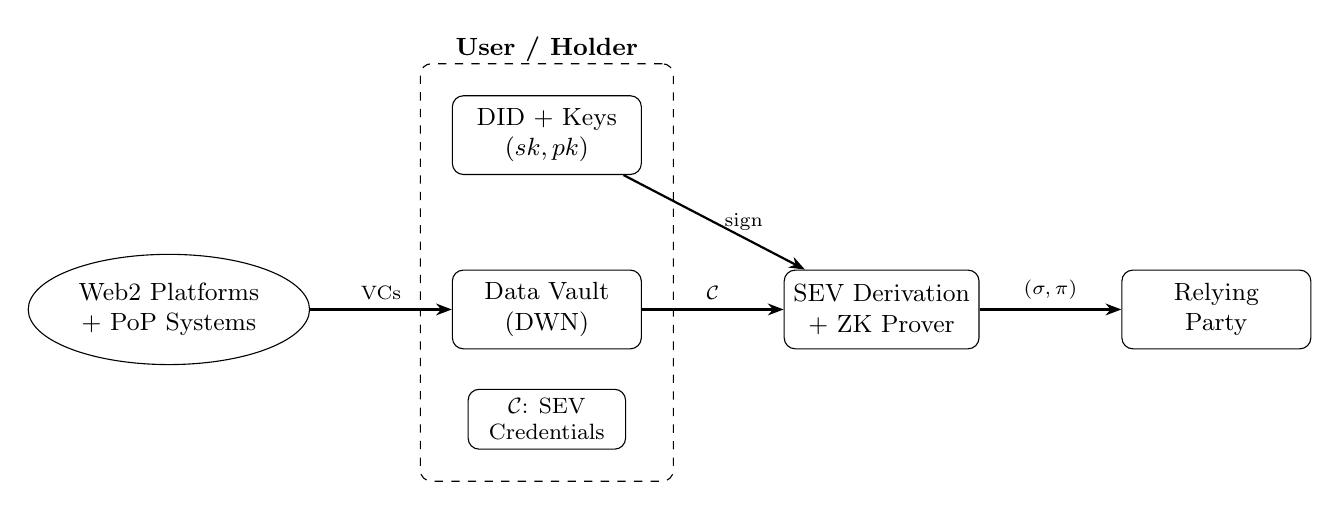
\begin{tikzpicture}[
    node distance=1.2cm and 1.8cm,
    box/.style={rectangle, draw, rounded corners, minimum width=2.4cm, minimum height=1cm, align=center, font=\small},
    smallbox/.style={rectangle, draw, rounded corners, minimum width=2cm, minimum height=0.7cm, align=center, font=\footnotesize},
    cloud/.style={ellipse, draw, minimum width=2.8cm, minimum height=1.4cm, align=center, font=\small},
    arrow/.style={-{Stealth[length=2mm]}, thick},
    label/.style={font=\scriptsize, align=center}
]

% Nodes
\node[cloud] (platforms) {Web2 Platforms\\+ PoP Systems};
\node[box, right=of platforms] (vault) {Data Vault\\(DWN)};
\node[smallbox, below=0.5cm of vault] (creds) {$\mathcal{C}$: SEV\\Credentials};
\node[box, above=of vault] (did) {DID + Keys\\$(sk, pk)$};
\node[box, right=of vault] (prover) {SEV Derivation\\+ ZK Prover};
\node[box, right=of prover] (rp) {Relying\\Party};

% User label
\node[above=0.3cm of did, font=\small\bfseries] (user) {User / Holder};

% Arrows
\draw[arrow] (platforms) -- node[above, label] {VCs} (vault);
\draw[arrow] (vault) -- node[above, label] {$\mathcal{C}$} (prover);
\draw[arrow] (did) -- node[right, label] {sign} (prover);
\draw[arrow] (prover) -- node[above, label] {$(\sigma, \pi)$} (rp);

% Dashed box around user-controlled components
\begin{scope}[on background layer]
\node[draw, dashed, rounded corners, inner sep=0.4cm, fit=(did)(vault)(creds), label={[font=\scriptsize]below:User-controlled}] {};
\end{scope}

\end{tikzpicture}
\caption{High-level SEL-DID architecture. The holder controls a DID and keys, stores SEV credentials $\mathcal{C}$ in a user-controlled data vault, derives $\mathcal{E}$ locally, and presents a DID signature $\sigma$ plus a ZK proof $\pi$ of policy satisfaction to relying parties.}
\label{fig:architecture}
\end{figure}

\subsection{Credential Issuance and SEV Construction}

We now describe how SEV-related credentials are issued and how the SEV is constructed.

\subsubsection{Platform-Level Credential Issuance}

For each platform $p \in \mathcal{P}$ that participates in SEL-DID evidence, we assume the existence of a credential schema $\mathsf{Schema}_p$ that specifies a reduced feature vector $\mathbf{y}_p$ derived from the raw activity $\mathbf{x}_p$. The goal of $\mathbf{y}_p$ is to retain useful information for Sybil-resistance and continuity while avoiding raw, identifying content.

An issuance interaction proceeds as follows:

\begin{enumerate}
  \item The holder authenticates to platform $p$ using the platform's native mechanism (e.g., OAuth, session cookie).
  \item The holder's SEL agent (running on their device) establishes a secure channel to $p$ and requests a SEV credential for their account, including their DID $\mathsf{did}$.
  \item Platform $p$ computes $\mathbf{x}_p$ over a trailing window $[t - \Delta, t]$, applies a public reduction function $r_p$ to obtain $\mathbf{y}_p = r_p(\mathbf{x}_p)$, and constructs a credential
  \[
    c_p = \big( \mathsf{id}_p, \mathsf{did}, \mathbf{y}_p, \textsf{meta}_p, \sigma_p \big),
  \]
  where $\mathsf{id}_p$ is a platform-specific pseudonymous account identifier, $\textsf{meta}_p$ contains issuance time and validity interval, and $\sigma_p$ is the platform's signature over the credential contents.
  \item The holder verifies $\sigma_p$ and, if valid, stores $c_p$ in their data vault, associating it with their SEL-DID.
\end{enumerate}

Credentials may have limited validity periods (e.g., 30--90 days), after which they must be refreshed. Revocation can be handled via standard VC revocation mechanisms (status lists, accumulators) or by short-lived credentials whose absence over time is treated as a signal of decay.

\subsubsection{Local SEV Aggregation}

Periodically, or on demand, the holder's SEL agent computes the SEV $\mathcal{E}$ from the set of currently valid credentials $\mathcal{C} = \{c_p\}$.

Let $\mathbf{y}_p$ denote the reduced feature vector in credential $c_p$. The agent computes:
\[
  \mathbf{y} = \bigoplus_{p \in \mathcal{P}'} \mathbf{y}_p,
\]
where $\mathcal{P}' \subseteq \mathcal{P}$ is the subset of platforms for which valid credentials are present.

The SEV is then:
\[
  \mathcal{E} = g(\mathbf{y}),
\]
where $g$ is a public transformation that may include normalization, dimensionality reduction, clipping, and quantization. The exact choice of $g$ is left to system designers and may differ between deployments; for example, a civic platform might choose a $g$ that emphasizes account age and local graph structure, while a developer-focused platform might weight contribution history more heavily.

The SEV $\mathcal{E}$ is maintained locally. Optionally, the holder may create an additional VC that commits to $\mathcal{E}$ via a cryptographic commitment:
\[
  \textsf{SEV\_VC} = \big( \mathsf{did}, \textsf{commit}(\mathcal{E}), \textsf{meta}, \sigma_{\mathsf{did}} \big),
\]
where $\sigma_{\mathsf{did}}$ is the holder's own signature. This can be useful for proving stability of $\mathcal{E}$ over time without recomputing from raw credentials.

\subsection{Passwordless Login with SEL-DIDs}

We now describe a passwordless login protocol in which a relying party (RP) authenticates a user based on:

\begin{enumerate}
  \item proof of control of the DID (standard DID Auth), and
  \item proof that the associated SEV satisfies a policy $\Pi$ chosen by the RP.
\end{enumerate}

\subsubsection{Policy Specification}

An RP specifies a SEL policy $\Pi$ as part of its authentication requirements. Examples include:

\begin{itemize}
  \item $\Pi_{\text{basic}}$: $C(t) \geq \tau_{\text{basic}}$, where $\tau_{\text{basic}}$ is a low threshold intended to filter out obvious burner identities.
  \item $\Pi_{\text{high}}$: $C(t) \geq \tau_{\text{high}}$ and ``SEV indicates at least $N$ independent platforms and account age $\geq A$ on two of them,'' intended for high-privilege operations.
\end{itemize}

We assume that $\Pi$ can be encoded as a predicate over $(\mathcal{E}, \mathcal{C})$ that is evaluable within the chosen ZK system.

\subsubsection{Authentication Flow}

Let $\mathsf{did}$ be the holder's SEL-DID, and let $(sk, pk)$ be the corresponding keypair.

The authentication protocol proceeds as follows:

\begin{enumerate}
  \item \textbf{Initialization.} The holder visits the RP and indicates a desire to log in using their SEL-DID. The RP responds with:
  \begin{itemize}
    \item a random challenge nonce $n$,
    \item a description of the SEL policy $\Pi$ it requires (e.g., $\Pi_{\text{basic}}$ or $\Pi_{\text{high}}$),
    \item the RP's verification parameters for the ZK proof system.
  \end{itemize}
  \item \textbf{Local proof preparation.} The holder's SEL agent:
  \begin{enumerate}
    \item retrieves the current set of valid credentials $\mathcal{C}$ and computes the current SEV $\mathcal{E}(t)$ and continuity score $C(t)$;
    \item checks locally whether $\Pi(\mathcal{E}(t), \mathcal{C})$ holds; if not, it can either abort or inform the user that the RP's policy cannot be met;
    \item constructs a ZK proof $\pi$ attesting that there exists $(\mathcal{E}, \mathcal{C})$ consistent with the committed SEV and credentials such that $\Pi(\mathcal{E}, \mathcal{C}) = 1$.
  \end{enumerate}
  \item \textbf{DID Auth.} In parallel or sequentially, the agent computes a signature $\sigma = \textsf{Sign}_{sk}(n \,\|\, \textsf{ctx})$, where $\textsf{ctx}$ binds the signature to this RP and session (e.g., includes the RP's domain and a timestamp).
  \item \textbf{Submission.} The holder sends to the RP:
  \[
    (\mathsf{did}, \sigma, \pi, \textsf{aux}),
  \]
  where $\textsf{aux}$ may include non-sensitive metadata such as the chosen SEL policy identifier and any public parameters needed to verify $\pi$.
  \item \textbf{Verification.} The RP:
  \begin{enumerate}
    \item resolves $\mathsf{did}$ to obtain the associated DID document $\mathsf{DD}$ and public key $pk$;
    \item verifies the signature $\sigma$ against $pk$ and challenge $n$;
    \item verifies the ZK proof $\pi$ against the policy $\Pi$ and the RP's verification parameters.
  \end{enumerate}
  If all checks pass, the RP accepts the authentication and establishes a session associated with $\mathsf{did}$ and the policy level used.
\end{enumerate}

This protocol provides passwordless authentication with two orthogonal assurances: key control and SEL policy satisfaction. The RP does not learn the specific platforms involved, the user's contacts, or detailed behavior, only that the SEV meets the specified criteria.

\subsection{Illustrative Login Flow}

Consider a user Alice with a SEL-DID backed by several long-lived accounts. Her SEL agent holds valid SEV credentials from three independent platforms and maintains a high continuity score $C(t)$.

When Alice logs into a DAO governance platform that enforces a high-assurance policy $\Pi_{\text{high}}$, the platform sends a challenge nonce and its policy description. Alice's agent:

\begin{enumerate}
  \item signs the nonce with the private key corresponding to her DID, and
  \item constructs a zero-knowledge proof that there exist SEV credentials $\mathcal{C}$ and a vector $\mathcal{E}$ such that $\Pi_{\text{high}}(\mathcal{E}, \mathcal{C}) = 1$ (for example: at least three independent platforms, two with age $\geq 3$ years, and $C(t) \geq \tau_{\text{high}}$).
\end{enumerate}

The DAO verifies the DID signature and the proof and admits the login. It never learns which platforms Alice used, how many followers she has, or what content she consumes; it only learns that this DID is backed by a high-entropy, long-lived behavioral profile satisfying its policy.

\subsection{Account Recovery with SEL-DIDs}

Account recovery in decentralized identity is notoriously difficult. SEL-DIDs offer additional levers by which recovery policies can be made both safer and more flexible.

We sketch a high-level recovery pattern; full formalization is left for future work.

\subsubsection{Recovery Goals}

We aim to enable a user who has lost access to the private key $sk$ associated with $\mathsf{did}$ to:

\begin{itemize}
  \item either bind a new keypair $(sk', pk')$ to the same DID (if the DID method supports key rotation under sufficient proof), or
  \item create a new DID $\mathsf{did}'$ and migrate their SEL layers in a way that relying parties can recognize as continuity of the same human.
\end{itemize}

At the same time, an attacker who has temporarily compromised some subset of the user's Web2 accounts should not be able to unilaterally perform such a recovery.

\subsubsection{Recovery Factors}

In addition to traditional recovery factors (e.g., social guardians, hardware backups), SEL-DID recovery policies can incorporate:

\begin{itemize}
  \item \textbf{Historical SEV continuity:} the requirement that the claimant can reconstruct a SEV $\mathcal{E}'$ with a continuity function $C'(t)$ that is consistent with the historical $C(t)$ associated with the original SEL-DID, over a sufficiently long window.
  \item \textbf{Multi-platform control:} the requirement that the claimant can obtain fresh SEV credentials from a threshold of independent platforms that were previously part of $\mathcal{C}$.
  \item \textbf{Time delays and community attestations:} the requirement that a recovery attempt be visible for some delay period and potentially co-signed by previously designated guardians or community members.
\end{itemize}

These factors raise the bar for an attacker who has compromised only a small subset of accounts or who cannot sustain a long-term imitation of behavior.

\subsubsection{Recovery Flow (Sketch)}

A generic recovery flow might proceed as follows:

\begin{enumerate}
  \item The user installs a new SEL agent and generates a fresh keypair $(sk', pk')$ and, if necessary, a new DID $\mathsf{did}'$.
  \item The agent re-establishes control over as many of the user's platforms as possible and obtains fresh credentials $\mathcal{C}'$ from them, constructing a new SEV $\mathcal{E}'$ and continuity score $C'(t)$.
  \item The agent initiates a recovery request to a recovery service or directly to relying parties, including:
  \begin{itemize}
    \item a proof that $\mathcal{E}'$ and $\mathcal{C}'$ are consistent with the historical SEV associated with the original SEL-DID (e.g., via overlapping account identifiers, long account ages, or ZK proofs of feature stability),
    \item proofs of control over additional recovery factors (guardians, hardware tokens, etc.),
    \item a binding statement that declares $\mathsf{did}'$ as the successor to the original $\mathsf{did}$.
  \end{itemize}
  \item After a policy-defined delay and verification process, RPs can choose to:
  \begin{itemize}
    \item update their internal records to treat $\mathsf{did}'$ as equivalent to the original $\mathsf{did}$, or
    \item accept logins from $\mathsf{did}'$ only if accompanied by stronger SEL proofs for a period of time.
  \end{itemize}
\end{enumerate}

We emphasize that SEL-DIDs do not require any particular global recovery coordinator; recovery policies can be implemented per-application or via shared registries. The key point is that the existence of a rich, long-term SEV and associated credentials allows recovery mechanisms to leverage behavioral continuity as an additional signal, beyond what is available in bare-key DID systems.

\section{Discussion: Privacy, Ethics, and Societal Implications}
\label{sec:discussion}

Using behavioral and social data to strengthen identity is inherently double-edged. The same signals that make Sybil attacks more expensive can, if misused, enable new forms of surveillance, exclusion, and control. In this section we discuss key privacy and ethical considerations for SEL-DIDs and outline design constraints intended to keep the framework aligned with human interests.

\subsection{Privacy and Data Minimization}

A primary design constraint for SEL-DIDs is that social and behavioral data must never be treated as key material. As stated in Section~\ref{sec:threat}, private keys remain high-entropy secrets under user control, and social entropy is layered on top via credentials and feature vectors. This avoids constructions in which compromise or replication of social data would directly compromise cryptographic control.

Even when social data is ``only'' used as evidence, the risk of privacy violations is significant. Raw activity traces---message contents, detailed contact graphs, precise timestamps---can reveal intimate details about a person's life. SEL-DIDs therefore rely on a combination of:

\begin{itemize}
  \item \textbf{Feature reduction.} Platforms and agents are expected to transform raw activity $\mathbf{x}_p$ into reduced vectors $\mathbf{y}_p$ that omit content and fine-grained identifiers, focusing instead on aggregate properties such as account age, interaction counts, and coarse-grained temporal patterns.
  \item \textbf{Quantization and bucketing.} Continuous features can be quantized into buckets (e.g., ``account older than three years'') to reduce linkability and make it harder to reconstruct precise histories from SEV proofs.
  \item \textbf{Zero-knowledge proofs and selective disclosure.} Relying parties should learn only that a predicate $\Pi(\mathcal{E}, \mathcal{C})$ holds, not the underlying coordinates of $\mathcal{E}$ or the list of platforms used.
\end{itemize}

These mechanisms are not a panacea; they must be continuously evaluated against evolving re-identification techniques. However, they provide a principled baseline: SEV-related credentials expose as little information as possible while still enabling useful Sybil-resistance and continuity signals.

\subsection{User Control and Storage}

Another requirement is that SEV-related credentials and any local representations of $\mathcal{E}$ reside in user-controlled data stores, such as Decentralized Web Nodes or equivalent personal data vaults. Centralized aggregation of raw behavioral logs into a single identity scoring service would undermine the core self-sovereign identity goals that DIDs were designed to support.

In the SEL-DID model, issuers (platforms, agents, or oracles) issue verifiable credentials to the user's vault; from there, all computation of $\mathcal{E}$ and generation of proofs occurs client-side. This reduces the attack surface and gives users the ability to:

\begin{itemize}
  \item rotate or split their identities across multiple DIDs,
  \item choose which credentials to present in which contexts,
  \item delete or revoke credentials when relationships with platforms change.
\end{itemize}

Ensuring that DWNs or equivalent vaults are themselves secure, resilient, and user-friendly is a substantial engineering and governance challenge, but it is orthogonal to SEL-DIDs and shared with the broader Web5 ecosystem.

\subsection{Inclusivity and Access}

Systems that reward ``high social entropy'' risk privileging already-privileged users: those with long-standing online presences, stable connectivity, and access to mainstream platforms. Conversely, people who are young, newly online, or deliberately low-profile may appear as low-entropy identities and thus face barriers to participation.

SEL-DIDs must therefore be designed with inclusivity in mind:

\begin{itemize}
  \item Participation in SEL layers must be optional; a DID without SEL evidence should still be usable in contexts that do not require Sybil resistance.
  \item Alternative evidence sources should be available for users with limited Web2 presence, such as local community attestations, offline proof-of-personhood ceremonies, or credentials issued by non-digital institutions.
  \item Policies $\Pi$ chosen by applications should be transparent and tunable, with clear trade-offs between Sybil resistance and inclusivity.
\end{itemize}

In particular, applications that serve vulnerable populations---such as people in conflict zones or under-resourced communities---should carefully calibrate their reliance on SEL-based proofs to avoid reinforcing existing inequities.

\subsection{Platform Dependence and Power}

Many of the richest behavioral signals today are held by large Web2 platforms. If SEL-DIDs were to depend heavily on these platforms as SEV issuers, the result could be a new form of platform lock-in: users with credentials from dominant platforms would enjoy stronger, more trusted identities, while others would be disadvantaged.

To mitigate this, SEL-DID deployments should:

\begin{itemize}
  \item treat any given Web2 platform as optional rather than mandatory;
  \item encourage a diversity of issuers, including smaller platforms, community-run services, and decentralized protocols;
  \item support issuance by user-controlled agents that compute features from data the user has already exported under data portability rights.
\end{itemize}

By designing SEV feature spaces and policies that can function without any single platform, SEL-DIDs can avoid quietly becoming ``Google plus friends'' under a different name.

\subsection{Platform Cooperation and Degradation}

In realistic deployments, most large Web2 platforms are unlikely to act as first-class SEV issuers. APIs are rate-limited or closed, business incentives favor data silos, and there is little reason for incumbents to strengthen identities outside their own ecosystems.

SEL-DIDs therefore assume a degraded, mixed environment by design. Where possible, user-controlled agents can compute $\mathbf{x}_p$ and $\mathbf{y}_p$ locally from data exports obtained under data portability rights (e.g., GDPR or CCPA), without requiring platforms to issue Verifiable Credentials directly. Where this is not possible, those platforms simply do not contribute to $\mathcal{E}$. Policies $\Pi$ are intended to be robust to such gaps: no single issuer is mandatory, and the system still functions (with weaker signals) when only a subset of a user's history can be incorporated.

\subsection{Abuse Scenarios and Misuse Risks}

If adopted widely, SEL-DIDs could be misused for purposes very different from Sybil resistance and privacy-preserving authentication. For example:

\begin{itemize}
  \item \textbf{Coercive identity scoring.} States or corporations could use SEV-like constructions to build opaque credit- or loyalty-scoring systems that condition access to services on behavioral conformity.
  \item \textbf{Surveillance.} Adversarial actors could pressure issuers or vault providers to reveal raw SEV inputs or to add hidden features that encode sensitive attributes.
  \item \textbf{Chilling effects.} If users believe that all their behavioral traces feed into a global identity score, they may self-censor or avoid legitimate but sensitive activities.
\end{itemize}

While no technical design alone can prevent such misuse, SEL-DIDs can be structured to make abusive deployments harder and more visible. For example, open standards bodies can:

\begin{itemize}
  \item restrict which kinds of features are considered acceptable in SEV schemas,
  \item require explicit disclosure of what policies $\Pi$ are being enforced and which issuers are trusted,
  \item encourage implementations that give users clear visibility into how their SEL evidence is used.
\end{itemize}

Ultimately, ethical deployment of SEL-DIDs will require not only technical safeguards but also governance, regulation, and informed public debate.

\subsection{Governance and Standardization}

Because SEL-DIDs build directly on DID and VC standards, they are natural candidates for discussion in the same standardization forums. Key open questions include:

\begin{itemize}
  \item how to represent SEV-related credentials and commitments in interoperable schemas;
  \item how to express policies $\Pi$ in a way that can be shared across applications and audited;
  \item how to certify or accredit SEV issuers, if at all, without centralizing power;
  \item how to expose sufficient metadata for users and auditors to understand the provenance and interpretation of SEL-based decisions.
\end{itemize}

Addressing these questions will determine whether SEL-DIDs remain an academic thought experiment or evolve into a practical, interoperable layer in the decentralized identity stack.

\subsection{Case Study: Civic Voting with Multi-Layer Verification}
\label{sec:case_study}

To illustrate how SEL-DIDs can be instantiated in practice, we describe a civic voting platform for local municipalities that achieves Sybil-resistant, location-verified voting without centralized identity oracles or biometric capture.

The system employs a four-layer verification model:

\begin{enumerate}
  \item \textbf{Basic authentication.} Users register via email, phone, or social login, establishing a persistent account anchor.
  \item \textbf{Social signature.} The platform aggregates signals from connected social accounts (e.g., activity history, account ages, cross-platform consistency) into a reputation score analogous to the SEV described in Section~\ref{sec:model}. This raises the cost of operating multiple fake accounts.
  \item \textbf{Financial stake OR high-entropy peer vouching.} Each vote requires \emph{either}:
  \begin{itemize}
    \item a small payment (e.g., \$1 equivalent), processed through a regulated payment provider that implicitly confirms possession of a local bank account, \emph{or}
    \item a cryptographic attestation (vouch) from a peer whose SEL-DID already exceeds a high-entropy threshold $\tau_{\text{vouch}}$ (e.g., $C(t) \geq 0.8$, multi-year presence on $\geq 3$ platforms).
  \end{itemize}
  The first option introduces economic friction without explicit KYC; the second provides an inclusion path for unbanked individuals while preserving Sybil resistance. Vouching is rate-limited: each high-entropy peer may vouch for at most $k$ new users per epoch (e.g., $k = 2$ per month), and a vouched user inherits a reduced initial standing until they independently accumulate sufficient entropy. This ensures that attackers cannot scale vouching without first building many expensive high-entropy identities.
  \item \textbf{Geographic verification.} At vote time, the user's device provides GPS coordinates, which are checked against municipality boundaries. The location is recorded on-chain alongside the vote hash, proving physical presence without revealing the user's home address.
\end{enumerate}

All votes are recorded on a public blockchain, enabling auditability while preserving ballot secrecy (the vote hash commits to the choice without revealing it until tabulation).

This design achieves several SEL-DID goals:

\begin{itemize}
  \item \textbf{Sybil resistance without biometrics.} An attacker wishing to cast $n$ fake votes must maintain $n$ aged social accounts, physically travel to the municipality $n$ times, and \emph{either} control $n$ local bank accounts and pay the per-vote fee $n$ times, \emph{or} cultivate enough high-entropy identities to vouch for $n$ accomplices (subject to rate limits). For modest $n$, this is already expensive; for large $n$, it is prohibitive.
  \item \textbf{No centralized identity oracle.} The system does not depend on a global uniqueness registry or a single issuer. Each verification layer is independent; failure or compromise of one layer degrades assurance but does not break the system.
  \item \textbf{Location-specific proof.} Unlike global proof-of-personhood schemes, the user only proves residency in a specific municipality, not worldwide uniqueness. This is sufficient for local governance and avoids the political and technical challenges of global identity.
  \item \textbf{Privacy-preserving.} The relying party (the voting platform) learns that a user satisfies the multi-layer policy, but does not see raw social graphs, financial balances, or precise home locations.
  \item \textbf{Inclusive by design.} The high-entropy peer vouching alternative ensures that unbanked individuals---who may lack access to regulated payment providers---are not excluded from civic participation. By allowing trusted community members to vouch for newcomers (subject to rate limits and entropy thresholds), the system preserves accessibility without compromising Sybil resistance.
\end{itemize}

This case study demonstrates that SEL-DIDs can be deployed incrementally, using existing infrastructure (social logins, payment processors, GPS), without waiting for new cryptographic ceremonies or biometric hardware. The approach is particularly suited to applications where geographic locality and moderate assurance are more relevant than global uniqueness guarantees.

\subsection{Limitations}
\label{sec:limitations}

SEL-DIDs inherit several structural limitations.

First, they suffer from a pronounced cold-start problem. New users, or users who have deliberately avoided persistent online traces, will naturally have low-entropy SEVs. For such users, SEL-based policies offer little advantage over bare-key authentication and may even be exclusionary if applied without care.

Second, aggregating behavioral features across platforms creates an inherent risk of correlation attacks. Even when $\mathbf{y}_p$ values are bucketed and only predicates $\Pi(\mathcal{E}, \mathcal{C})$ are revealed, an adversary observing multiple interactions might progressively narrow down which platforms and behavioral profiles are likely. Mitigation requires conservative feature design, coarse bucketing, and potentially differential privacy; a full analysis is left to future work.

Third, temporal attacks exploiting markets for aged accounts remain a real concern. Black markets already trade in ``seasoned'' social accounts with long histories and plausible graphs. SEL-DIDs do not eliminate this, but they can raise the bar: policies can weight recent behavioral consistency, require evidence from multiple independent platforms, and emphasize features that are harder to fake at scale (e.g., long-lived conversational ties across contexts). For high-value applications, SEL-based signals should be combined with other factors such as stake, social attestations, or in-person ceremonies.

\section{Conclusion}

Decentralized Identifiers promise self-sovereign identity by allowing users to generate and control their own identifiers and keys without centralized registries. In practice, however, bare DIDs leave open three central challenges: Sybil resistance, continuity and recovery, and trust bootstrapping for passwordless authentication. At the same time, most people already generate rich, long-lived behavioral traces across multiple platforms that, if used carefully, can raise the cost of forging convincing identities at scale.

This paper introduced \emph{Social Entropy Layered DIDs} (SEL-DIDs), a model in which a conventional DID and keypair form the cryptographic root of identity, and cross-platform behavioral and social evidence is attached as an optional, user-controlled layer. We formalized the notion of a Social Entropy Vector (SEV) $\mathcal{E}$ derived from per-platform feature vectors, and described how SEV-related credentials can be issued as Verifiable Credentials and stored in personal data vaults such as Decentralized Web Nodes. We presented a threat model and design goals for SEL-DIDs focused on Sybil-resistance amplification, key-compromise damage limitation, platform-agnostic continuity, privacy-preserving verification, and passwordless authentication with recovery.

On top of this model, we outlined a cryptographic construction and a passwordless login protocol in which relying parties verify both control of the DID and satisfaction of a SEL policy $\Pi$ over the SEV, using zero-knowledge proofs or selective disclosure. We sketched how the same machinery can support safer recovery flows by leveraging historical SEV continuity and multi-platform control as recovery factors, without turning any single platform into a mandatory oracle. Finally, we analyzed privacy, ethical, and societal implications of using behavioral data as identity-strengthening evidence, emphasizing data minimization, user-controlled storage, inclusivity, and the need to avoid new forms of platform lock-in or coercive identity scoring.

This work is intentionally architectural rather than empirical. We do not claim to have solved the full problem of proof-of-personhood or to have calibrated a definitive cost-of-forgery model for Social Entropy Vectors. Important directions for future work include: (i) designing concrete SEV feature spaces and reduction functions $r_p$ that balance utility against privacy; (ii) empirically evaluating SEL-based policies on real or synthetic datasets to estimate adversary costs and false-positive rates; (iii) integrating existing proof-of-personhood systems (e.g., BrightID, Gitcoin Passport) as inputs into SEV constructions; (iv) specifying interoperable schemas and policy languages for SEL credentials within existing DID and VC standards; and (v) prototyping SEL-DIDs in real-world applications such as governance platforms, Sybil-resistant funding mechanisms, and civic networks.

If these challenges can be addressed, SEL-DIDs offer a path toward decentralized identities that are not only self-sovereign in a cryptographic sense, but also resistant to large-scale forgery, recoverable in practice, and compatible with privacy-preserving, passwordless authentication. Rather than replacing cryptographic keys with social data, SEL-DIDs treat social and behavioral entropy as a layered, revocable signal under user control, giving applications more nuanced tools to reason about human identities in decentralized systems.

\bibliographystyle{plain}
\bibliography{sel-did}

\end{document}
